\documentclass[10pt]{report}
\usepackage[table]{xcolor}    % loads also »colortbl«. MUST BE LOADED FIRST
\usepackage[utf8]{inputenc}
\usepackage{csquotes}
\usepackage[english]{babel}
\usepackage{ngtrigger}
\usepackage{lipsum} % For dummy text
\usepackage[
backend=biber,
style=numeric,
sorting=ynt
]{biblatex}
\usepackage{hyperref}                % For clickable hyperlinks
\usepackage{siunitx}
\usepackage{href-ul}
\usepackage{tcolorbox}
\usepackage{longtable}
\usepackage{booktabs}  % For \toprule, \midrule, \bottomrule
\usepackage{array}     % For defining custom column types
\usepackage{multirow}  % For spanning multiple rows and cols
\usepackage{svg}
\usepackage{graphicx}
\usepackage{adjustbox}

\setcounter{tocdepth}{3}  % Include subsubsections in the TOC

\usepackage{listings}
\usepackage{xcolor}  % For syntax highlighting colors (optional)

% Custom symbols
\newcommand{\pbinv}{\ensuremath{\mathrm{pb}^{-1}}}
\newcommand{\fbinv}{\ensuremath{\mathrm{fb}^{-1}}}
\newcommand{\kHz}{\ensuremath{\,\mathrm{kHz}}}

% Custom configuration for code appearance
\lstset{
    basicstyle=\ttfamily\footnotesize,  % Basic font settings
    keywordstyle=\color{blue},          % Keyword color
    commentstyle=\color{green!60!black},% Comment color
    stringstyle=\color{red},            % String color
    numbers=left,                       % Line numbers on the left
    numberstyle=\tiny\color{gray},      % Line number font and color
    stepnumber=1,                       % Number every line
    tabsize=4,                          % Tab spaces
    breaklines=true,                    % Break long lines
    frame=single,                       % Draw a frame around the code
}

% Define a new column type for \texttt (monospaced font)
\newcolumntype{T}{>{\ttfamily}l}  % "T" is the new column type, "l" for left alignment
% Define a new column type for \texttt (monospaced font) that uses 60% of the available space
\newcolumntype{Z}{>{\ttfamily\raggedright\hspace{0pt}}p{0.6\textwidth}}

% Prepare content for the title page
\author{Marco Musich, Jessica Prendi, Thiago Tomei, Mateusz Zarucki}
\title{Optimal HLT Calibrations}
\subtitle{NGT Task 3.4 2024 Report}

% Start chapter from 1
\setcounter{chapter}{0}
% Start section from 1
\setcounter{section}{0}

\addbibresource{references.bib}      % Reference your .bib file

% Declate new siunitx
\DeclareSIUnit{\event}{ev}
\DeclareSIUnit{\CHF}{CHF}
\DeclareSIUnit{\HS}{HS23}

\begin{document}

% Load colors from Tang palette, among many others.
%{{{ TANGO PALETTE
% butter
\definecolor{butter1}{rgb}{0.9882352941176471, 0.9137254901960784, 0.30980392156862746}% #FCE94F
\definecolor{butter2}{rgb}{0.92941176470588238, 0.83137254901960789, 0.0}% #EDD400
\definecolor{butter3}{rgb}{0.7686274509803922, 0.62745098039215685, 0.0}% #C4A000
% orange
\definecolor{orange1}{rgb}{0.9882352941176471, 0.68627450980392157, 0.24313725490196078} % #FCAF3E
\definecolor{orange2}{rgb}{0.96078431372549022, 0.47450980392156861, 0.0} % #F57900
\definecolor{orange3}{rgb}{0.80784313725490198, 0.36078431372549019, 0.0} % #CE5C00
% chocolate
\definecolor{chocolate1}{rgb}{0.9137254901960784, 0.72549019607843135, 0.43137254901960786} % #E9B96E
\definecolor{chocolate2}{rgb}{0.75686274509803919, 0.49019607843137253, 0.066666666666666666} % #C17D11
\definecolor{chocolate3}{rgb}{0.5607843137254902, 0.34901960784313724, 0.0078431372549019607} % #8F5902
% chameleon
\definecolor{chameleon1}{rgb}{0.54117647058823526, 0.88627450980392153, 0.20392156862745098} % #8AE234
\definecolor{chameleon2}{rgb}{0.45098039215686275, 0.82352941176470584, 0.086274509803921567} % #73D216
\definecolor{chameleon3}{rgb}{0.30588235294117649, 0.60392156862745094, 0.023529411764705882} % #4E9A06
% sky blue
\definecolor{skyblue1}{rgb}{0.44705882352941179, 0.62352941176470589, 0.81176470588235294} % #729FCF
\definecolor{skyblue2}{rgb}{0.20392156862745098, 0.396078431372549, 0.64313725490196083} % #3465A4
\definecolor{skyblue3}{rgb}{0.12549019607843137, 0.29019607843137257, 0.52941176470588236} % #204A87
% plum
\definecolor{plum1}{rgb}{0.67843137254901964, 0.49803921568627452, 0.6588235294117647} % #AD7FA8
\definecolor{plum2}{rgb}{0.45882352941176469, 0.31372549019607843, 0.4823529411764706} % #75507B
\definecolor{plum3}{rgb}{0.36078431372549019, 0.20784313725490197, 0.40000000000000002} % #5C3566
% scarlet red
\definecolor{scarletred1}{rgb}{0.93725490196078431, 0.16078431372549021, 0.16078431372549021} % #EF2929
\definecolor{scarletred2}{rgb}{0.80000000000000004, 0.0, 0.0} % #CC0000
\definecolor{scarletred3}{rgb}{0.64313725490196083, 0.0, 0.0} % #A40000
% aluminium
\definecolor{aluminium1}{rgb}{0.93333333333333335, 0.93333333333333335, 0.92549019607843142} % #EEEEEC
\definecolor{aluminium2}{rgb}{0.82745098039215681, 0.84313725490196079, 0.81176470588235294} % #D3D7CF
\definecolor{aluminium3}{rgb}{0.72941176470588232, 0.74117647058823533, 0.71372549019607845} % #BABDB6
% gray
\definecolor{gray1}{rgb}{0.53333333333333333, 0.54117647058823526, 0.52156862745098043} % #888A85
\definecolor{gray2}{rgb}{0.33333333333333331, 0.3411764705882353, 0.32549019607843138} % #555753
\definecolor{gray3}{rgb}{0.1803921568627451, 0.20392156862745098, 0.21176470588235294} % #2E3436
%}}}

%{{{ SOLARIZED PALETTE
\definecolor{sol-base03}{rgb}{0.,0.16862,0.21176}
\definecolor{sol-base02}{rgb}{0.02745,0.21176,0.25882}
\definecolor{sol-base01}{rgb}{0.34509,0.43137,0.45882}
\definecolor{sol-base00}{rgb}{0.39607,0.48235,0.51372}
\definecolor{sol-base0}{rgb}{0.51372,0.58039,0.58823}
\definecolor{sol-base1}{rgb}{0.57647,0.63137,0.63137}
\definecolor{sol-base2}{rgb}{0.93333,0.90980,0.83529}
\definecolor{sol-base3}{rgb}{0.99215,0.96470,0.89019}
\definecolor{sol-yellow}{rgb}{0.70980,0.53725,0.}
\definecolor{sol-orange}{rgb}{0.79607,0.29411,0.08627}
\definecolor{sol-red}{rgb}{0.86274,0.19607,0.18431}
\definecolor{sol-magenta}{rgb}{0.82745,0.21176,0.50980}
\definecolor{sol-violet}{rgb}{0.42352,0.44313,0.76862}
\definecolor{sol-blue}{rgb}{0.1490,0.54509,0.82352}
\definecolor{sol-cyan}{rgb}{0.16470,0.63137,0.59607}
\definecolor{sol-green}{rgb}{0.52156,0.6,0.}
%}}}

%{{{ TIMELINECOLORS
\colorlet{tlc0}{skyblue1}
\colorlet{tlc1}{chameleon1}
\colorlet{tlc2}{sol-red}
\colorlet{tlc3}{butter2}
\colorlet{tlc4}{chameleon1}
\colorlet{tlc5}{skyblue2}
\colorlet{tlc6}{plum1}
\colorlet{tlc7}{orange1}
\colorlet{tlc8}{chameleon1}
\colorlet{tlc9}{butter2}
\colorlet{tlc10}{tlc0}
\colorlet{tlc11}{tlc1}
\colorlet{tlc12}{tlc2}
\colorlet{tlc13}{tlc3}
\colorlet{tlc14}{tlc4}
\colorlet{tlc15}{tlc5}
\colorlet{tlc16}{tlc6}
\colorlet{tlc17}{tlc7}
\colorlet{tlc18}{tlc8}
\colorlet{tlc19}{tlc9}
%}}}

%{{{ FROM CERN LOGO
\definecolor{palette1}{rgb}{0.016,0.157,0.380} %(214,214,241)
\definecolor{palette2}{rgb}{0.13,0.29,0.61} % Blue LOGO CERN
\definecolor{palette3}{rgb}{0.17,0.39,0.81} % Blue LOGO CERN derived
%}}}

%{{{ MISCELLANEA
\definecolor{exampleblock}{rgb}{0.27,0.68,0.03}   % verde exampleblock
\definecolor{exampleblockbody}{rgb}{0.89,0.98,0.83}   % verde exampleblock
\definecolor{alertC}{rgb}{0.878,0.137,0.035}

\definecolor{blueScuro}{rgb}{0.04,0.04,0.278} % 0A0A47
\definecolor{titleWhite}{rgb}{0.949, 0.941, 0.941}
\definecolor{alertCTitle}{rgb}{0.651, 0.059, 0.059}
%}}}

%{{{ %%%%%%% NEW BLUE %%%%%%%% from colorTable_26_26_89.html
\definecolor{blue1}{rgb}{0.035,0.361,0.878}           % Chiaro - Titolo
\definecolor{blue3}{rgb}{0.027,0.278,0.678}          % Medio Scuro
\definecolor{blue2}{rgb}{0.016,0.157,0.380}          % Scuro
\definecolor{alertCTitle}{rgb}{0.878,0.137,0.035}
\definecolor{ppblue}  {rgb}{0.824,0.980,0.843} %  from colorTable_0_255_70.html
\definecolor{ppgreen} {rgb}{0.980,0.929,0.922} %  from colorTable_0_255_70.html
\definecolor{blue2a}{rgb}{0.16, 0.1, 0.35} %
\definecolor{blue2b}{rgb}{0.22, 0.1, 0.35} %
\definecolor{blue2c}{rgb}{0.29, 0.1, 0.35} %
\definecolor{blue2d}{rgb}{0.35, 0.1, 0.35} %
\definecolor{blue2A}{rgb}{0.1, 0.16, 0.35} %
\definecolor{blue2B}{rgb}{0.10, 0.22, 0.35} %
\definecolor{blue2C}{rgb}{0.10, 0.29, 0.35} %
\definecolor{blue2D}{rgb}{0.1, 0.35, 0.35} %
\definecolor{ppred}  {rgb}{1     , 0.796 , 0.937} % FF CB EF pale pale red
\definecolor{pgreen} {rgb}{0.835 , 1     , 0.796} % D5 FF CB pale green
\definecolor{pred}   {rgb}{1     , 0.796 , 0.835} % FF CB D5 pale red
\definecolor{pblue}  {rgb}{0.796 , 0.835 , 1    } % CB D5 FF pale blue
%}}}

%{{{ COMMENTED OUT

%{{{ %%%%%% BLUE %%%%%%%%%% from colorTable_34_34_115.html
%\definecolor{blue1}{rgb}{0.251,0.251,0.851}           % Chiaro - Titolo (rot 0 bal 30/40)
%\definecolor{blue3}{rgb}{0.192,0.192,0.651}          % Medio Scuro (rot 0 bal 20)
%\definecolor{blue2}{rgb}{0.102,0.102,0.349}          % Scuro (rot 0 bal -10)
%\definecolor{exampleblock}{rgb}{0.651,0.192,0.651}   % verde exampleblock (rot 60 bal 20)
%\definecolor{alertC}{rgb}{0.251,0.851,0.851}         % (rot -60 bal 40)
%\definecolor{alertCTitle}{rgb}{0.251,0.851,0.851}
%%  from colorTable built using rot 0 bal 50 of previous table
%\definecolor{ppblue}  {rgb}{0.949,0.855,0.949} %
%\definecolor{ppgreen} {rgb}{0.855,0.925,0.949} % rot 60 sat 60
%}}}
%{{{%%%%%%% ORIGINAL BLUE %%%%%%%% from colorTable_26_26_89.html
%\definecolor{blue1}{rgb}{0.247,0.247,0.851}           % Chiaro - Titolo
%\definecolor{blue3}{rgb}{0.161,0.161,0.549}          % Medio Scuro
%\definecolor{blue2}{rgb}{0.102,0.102,0.349}          % Scuro
%\definecolor{exampleblock}{rgb}{0.000,0.502,0.012}   % verde exampleblock
%\definecolor{alertC}{rgb}{0.949,0.086,0.086}
%\definecolor{alertCTitle}{rgb}{0.651,0.059,0.059}
%\definecolor{ppblue}  {rgb}{0.800,0.945,1.000} %  from colorTable_0_255_70.html
%\definecolor{ppgreen} {rgb}{0.800,1.000,0.804} %  from colorTable_0_255_70.html
%}}}
%{{{%%%%% ORANGE %%%%%%%%% from colorTable_153_38_0.html
%\definecolor{blue1}{rgb}{0.902,0.447,0.000}         % Chiaro - Titolo
%\definecolor{blue3}{rgb}{0.800,0.396,0.000}         % Medio Scuro
%\definecolor{blue2}{rgb}{0.502,0.251,0.000}         % Scuro
%\definecolor{exampleblock}{rgb}{0.353,0.698,0.000}  % verde exampleblock
%\definecolor{alertC}{rgb}{0.698,0.000,0.353}
%\definecolor{alertCTitle}{rgb}{0.698,0.000,0.353}
%%  from colorTable built using rot 0 bal 50 of previous table
%\definecolor{ppblue}  {rgb}{0.953,1.000,0.902} %  rot 60 sat -90
%\definecolor{ppgreen} {rgb}{1.000,0.902,0.953} %  rot -60 sat -90
%}}}
%{{{%%%%% ORANGE %%%%%%%%% from colorTable_255_0_0.html
%\definecolor{blue1}{rgb}{0.902,0.451,0.000}         % Chiaro - Titolo
%\definecolor{blue3}{rgb}{0.698,0.173,0.000}         % Medio Scuro
%\definecolor{blue2}{rgb}{0.502,0.125,0.000}         % Scuro
%\definecolor{exampleblock}{rgb}{0.000,0.502,0.012}  % verde exampleblock
%\definecolor{alertC}{rgb}{0.800,0.000,0.000}
%\definecolor{alertCTitle}{rgb}{0.800,0.000,0.000}
%%  from colorTable built using rot 0 bal 50 of previous table
%\definecolor{ppblue}  {rgb}{0.800,0.945,1.000} %  from colorTable_0_255_70.html
%\definecolor{ppgreen} {rgb}{0.800,1.000,0.804} %  from colorTable_0_255_70.html
%}}}
%{{{%%%%%% GREEN %%%%%%%%%% from colorTable_8_89_8.html
%\definecolor{blue1}{rgb}{0.059,0.651,0.059}           % Chiaro - Titolo
%\definecolor{blue3}{rgb}{0.051,0.549,0.051}           % Medio Scuro
%\definecolor{blue2}{rgb}{0.024,0.251,0.024}           % Scuro
%\definecolor{exampleblock}{rgb}{0.051,0.549,0.549}    % verde exampleblock
%\definecolor{alertC}{rgb}{0.749,0.749,0.067}
%\definecolor{alertCTitle}{rgb}{0.749,0.749,0.067}
%\definecolor{ppblue}  {rgb}{0.800,0.945,1.000} %  from colorTable_0_255_70.html
%\definecolor{ppgreen} {rgb}{0.800,1.000,0.804} %  from colorTable_0_255_70.html
%}}}
%{{{%%%%%% New BLUE %%%%%%%%%% from colorTable_34_34_115.html
%\definecolor{blue1}{rgb}{0.231,0.545,0.741}           % Chiaro - Titolo (rot 0 bal 30/40)
%\definecolor{blue3}{rgb}{0.169,0.396,0.541}          % Medio Scuro (rot 0 bal 20)
%\definecolor{blue2}{rgb}{0.075,0.176,0.239}          % Scuro (rot 0 bal -10)
%\definecolor{exampleblock}{rgb}{0.424,0.231,0.741}   % verde exampleblock (rot 60 bal 20)
%\definecolor{alertC}{rgb}{0.231,0.741,0.427}         % (rot -60 bal 40)
%\definecolor{alertCTitle}{rgb}{0.231,0.741,0.427}
%%  from colorTable built using rot 0 bal 50 of previous table
%\definecolor{ppblue}  {rgb}{0.745,0.682,0.843} %
%\definecolor{ppgreen} {rgb}{0.682,0.843,0.745} % rot 60 sat 60
%}}}

%}}}

%{{{ OTHERS
%\colorlet{redshaded}{red!25!bg}
%\colorlet{shaded}{black!25!bg}
%\colorlet{shadedshaded}{black!10!bg}
%\colorlet{blackshaded}{black!40!bg}

%\colorlet{darkred}{red!30!black}
%\colorlet{darkblue}{blue!30!black}
%\colorlet{darkgreen}{green!30!black}


\def\radius{0.96cm}
\def\innerradius{0.85cm}

\def\softness{0.4}
\definecolor{softred}{rgb}{1,\softness,\softness}
\definecolor{softgreen}{rgb}{\softness,1,\softness}
\definecolor{softblue}{rgb}{\softness,\softness,1}

\definecolor{softrg}{rgb}{1,1,\softness}
\definecolor{softrb}{rgb}{1,\softness,1}
\definecolor{softgb}{rgb}{\softness,1,1}

\def\softsoftness{0.9}
\definecolor{softsoftred}{rgb}{1,\softsoftness,\softsoftness}
\definecolor{softsoftgreen}{rgb}{\softsoftness,1,\softsoftness}
\definecolor{softsoftblue}{rgb}{\softsoftness,\softsoftness,1}

\definecolor{QuestionSlide}{RGB}{49,106,255}
\definecolor{beamer@blendedblue}{rgb}{0.23,0.4,0.7}% use structure theme to change
%}}}

%{{{ CERN
\definecolor{cern}{RGB}{0,51,160}
\definecolor{ukrb}{RGB}{0,87,183}
\definecolor{ukry}{RGB}{255,215,0}
%}}}



% Set alternating color for rows in tables
\rowcolors*[]{2}{aluminium1!50!white}{white}
%
%% Add newly defined newly defined commands.
\newcommand{\ngt}{\textsf{NGT}}
\newcommand{\task}[1]{\textsf{Task #1}}
\newcommand{\soa}{\textsf{SoA}}
\newcommand{\hltp}{\texttt{HLT Phase\num{2}}}
\newcommand{\offp}{\texttt{Offline Phase\num{2}}}
\newcommand{\run}[1]{Run-\num{#1}}
\newcommand{\hs}[1]{\texttt{HS#1}}
\newcommand{\Lone}{Level-\num{1}}
\NewDocumentCommand {\CMSSW} { s O{X} O{X} O{X} o} {%
  \IfBooleanTF {#1}
  {%
    \textsc{CMSSW}%
  }%
  {
    \IfNoValueTF {#5}
    {%
      \textsc{CMSSW}\_{#2}\_{#3}\_{#4}%
    }%
    {
      \textsc{CMSSW}\_{#2}\_{#3}\_{#4}\_pre{#5}%
    }%
  }%
}%

% Define a colorbox for a NotaBene clarification
\newtcolorbox{nbbox}{%
  colback=yellow!10!white,
  colframe=yellow!80!black,
  fonttitle=\sffamily\bfseries,
  title=Nota Bene}
 
% Define a colorbox for an Alert clarification
\newtcolorbox{alertbox}{%
  colback=scarletred1!10!white,
  colframe=scarletred3!80!black,
  fonttitle=\sffamily\bfseries,
  title=Alert}
\newcommand{\Hz}{\ensuremath{\,\text{Hz}}\xspace}
\newcommand{\kHz}{\ensuremath{\,\text{kHz}}\xspace}
\newcommand{\MHz}{\ensuremath{\,\text{MHz}}\xspace}
\newcommand{\Tb}{\ensuremath{\,\text{Tb}}\xspace}
\newcommand{\Tbpers}{\ensuremath{\,\text{Tb/s}}\xspace}
\newcommand{\Gb}{\ensuremath{\,\text{Gb}}\xspace}
\newcommand{\Gbpers}{\ensuremath{\,\text{Gb/s}}\xspace}
\newcommand{\Mbpers}{\ensuremath{\,\text{Mb/s}}\xspace}
\newcommand{\Mb}{\ensuremath{\,\text{Mb}}\xspace}
%% Not pretty, but have to work around a conflict with pennames also
%% defining \PB. Not likely both definitions will be used in the same
%% document (if using \renewcommand)
\newcommand{\PB}{\ensuremath{\,\text{PB}}\xspace}
\newcommand{\TB}{\ensuremath{\,\text{TB}}\xspace}
\newcommand{\GB}{\ensuremath{\,\text{GB}}\xspace}
\newcommand{\GBpers}{\ensuremath{\,\text{GB/s}}\xspace}
\newcommand{\MB}{\ensuremath{\,\text{MB}}\xspace}
\newcommand{\Runone}{\run{1}\xspace}
\newcommand{\Runtwo}{\run{2}\xspace}
\newcommand{\Runthree}{\run{3}\xspace}
\newcommand{\Runfour}{\run{4}\xspace}
\newcommand{\Runfive}{\run{5}\xspace}
\newcommand{\Phasezero}{\text{\mbox{Phase-0}}\xspace}
\newcommand{\Phaseone}{\text{\mbox{Phase-1}}\xspace}
\newcommand{\Phasetwo}{\text{\mbox{Phase-2}}\xspace}
\newcommand{\pileup}{$\langle{\rm PU}\rangle$\xspace}
\newcommand{\pileupof}[1]{$\langle{\rm PU}\rangle = #1$\xspace}

%%% Copied from ptdr-definitions.sty
% Measurements and units...

\newcommand{\de}{\ensuremath{^\circ}}
\newcommand{\ten}[1]{\ensuremath{\times \text{10}^\text{#1}}}
%\newcommand{\unit}[1]{\ensuremath{\text{\,#1}}\xspace}
\newcommand{\mum}{\ensuremath{\,\mu\text{m}}\xspace}
\newcommand{\micron}{\ensuremath{\,\mu\text{m}}\xspace}
\newcommand{\cm}{\ensuremath{\,\text{cm}}\xspace}
\newcommand{\mm}{\ensuremath{\,\text{mm}}\xspace}
\newcommand{\mus}{\ensuremath{\,\mu\text{s}}\xspace}
\newcommand{\keV}{\ensuremath{\,\text{ke\hspace{-.08em}V}}\xspace}
\newcommand{\MeV}{\ensuremath{\,\text{Me\hspace{-.08em}V}}\xspace}
\newcommand{\MeVns}{\ensuremath{\text{Me\hspace{-.08em}V}}\xspace} % no leading thinspace
\newcommand{\GeV}{\ensuremath{\,\text{Ge\hspace{-.08em}V}}\xspace}
\newcommand{\GeVns}{\ensuremath{\text{Ge\hspace{-.08em}V}}\xspace} % no leading thinspace
\newcommand{\gev}{\GeV}
\newcommand{\TeV}{\ensuremath{\,\text{Te\hspace{-.08em}V}}\xspace}
\newcommand{\TeVns}{\ensuremath{\text{Te\hspace{-.08em}V}}\xspace} % no leading thinspace
\newcommand{\PeV}{\ensuremath{\,\text{Pe\hspace{-.08em}V}}\xspace}
\newcommand{\keVc}{\ensuremath{{\,\text{ke\hspace{-.08em}V\hspace{-0.16em}/\hspace{-0.08em}}c}}\xspace}
\newcommand{\MeVc}{\ensuremath{{\,\text{Me\hspace{-.08em}V\hspace{-0.16em}/\hspace{-0.08em}}c}}\xspace}
\newcommand{\GeVc}{\ensuremath{{\,\text{Ge\hspace{-.08em}V\hspace{-0.16em}/\hspace{-0.08em}}c}}\xspace}
\newcommand{\GeVcns}{\ensuremath{{\text{Ge\hspace{-.08em}V\hspace{-0.16em}/\hspace{-0.08em}}c}}\xspace} % no leading thinspace
\newcommand{\TeVc}{\ensuremath{{\,\text{Te\hspace{-.08em}V\hspace{-0.16em}/\hspace{-0.08em}}c}}\xspace}
\newcommand{\keVcc}{\ensuremath{{\,\text{ke\hspace{-.08em}V\hspace{-0.16em}/\hspace{-0.08em}}c^\text{2}}}\xspace}
\newcommand{\MeVcc}{\ensuremath{{\,\text{Me\hspace{-.08em}V\hspace{-0.16em}/\hspace{-0.08em}}c^\text{2}}}\xspace}
\newcommand{\GeVcc}{\ensuremath{{\,\text{Ge\hspace{-.08em}V\hspace{-0.16em}/\hspace{-0.08em}}c^\text{2}}}\xspace}
\newcommand{\GeVccns}{\ensuremath{{\text{Ge\hspace{-.08em}V\hspace{-0.16em}/\hspace{-0.08em}}c^\text{2}}}\xspace} % no leading thinspace
\newcommand{\TeVcc}{\ensuremath{{\,\text{Te\hspace{-.08em}V\hspace{-0.16em}/\hspace{-0.08em}}c^\text{2}}}\xspace}

\newcommand{\abinv} {\mbox{\ensuremath{\,\text{ab}^{-1}}}\xspace}
\newcommand{\fbinv} {\mbox{\ensuremath{\,\text{fb}^{-1}}}\xspace}
\newcommand{\pbinv} {\mbox{\ensuremath{\,\text{pb}^{-1}}}\xspace}
\newcommand{\nbinv} {\mbox{\ensuremath{\,\text{nb}^{-1}}}\xspace}
\newcommand{\mubinv} {\ensuremath{\,\mu\text{b}^{-1}}\xspace}
\newcommand{\mbinv} {\ensuremath{\,\text{mb}^{-1}}\xspace}
\newcommand{\percms}{\ensuremath{\,\text{cm}^{-2}\,\text{s}^{-1}}\xspace}
\newcommand{\lumi}{\ensuremath{\mathcal{L}}\xspace}
\newcommand{\Lumi}{\ensuremath{\mathcal{L}}\xspace}%both upper and lower
%
% Need a convention here:
\newcommand{\LvLow}  {\ensuremath{\mathcal{L}=\text{10}^\text{32}\,\text{cm}^\text{$-$2}\,\text{s}^\text{$-$1}}\xspace}
\newcommand{\LLow}   {\ensuremath{\mathcal{L}=\text{10}^\text{33}\,\text{cm}^\text{$-$2}\,\text{s}^\text{$-$1}}\xspace}
\newcommand{\lowlumi}{\ensuremath{\mathcal{L}=\text{2}\times \text{10}^\text{33}\,\text{cm}^\text{$-$2}\,\text{s}^\text{$-$1}}\xspace}
\newcommand{\LMed}   {\ensuremath{\mathcal{L}=\text{2}\times \text{10}^\text{33}\,\text{cm}^\text{$-$2}\,\text{s}^\text{$-$1}}\xspace}
\newcommand{\LHigh}  {\ensuremath{\mathcal{L}=\text{10}^\text{34}\,\text{cm}^\text{$-$2}\,\text{s}^\text{$-$1}}\xspace}
\newcommand{\hilumi} {\ensuremath{\mathcal{L}=\text{10}^\text{34}\,\text{cm}^\text{$-$2}\,\text{s}^\text{$-$1}}\xspace}

% Physics symbols ...

\newcommand{\PT}{\ensuremath{p_{\mathrm{T}}}\xspace}
\newcommand{\pt}{\ensuremath{p_{\mathrm{T}}}\xspace}
\newcommand{\ET}{\ensuremath{E_{\mathrm{T}}}\xspace}
\newcommand{\HT}{\ensuremath{H_{\mathrm{T}}}\xspace}
\newcommand{\mT}{\ensuremath{m_{\mathrm{T}}}\xspace}
\newcommand{\mTii}{\ensuremath{m_{\mathrm{T2}}}\xspace}
\newcommand{\et}{\ensuremath{E_{\mathrm{T}}}\xspace}
\newcommand{\Em}{\ensuremath{E\hspace{-0.6em}/}\xspace}
\newcommand{\Pm}{\ensuremath{p\hspace{-0.5em}/}\xspace}
\newcommand{\PTm}{\ensuremath{{p}_\mathrm{T}\hspace{-1.02em}/\kern 0.5em}\xspace}
\newcommand{\PTslash}{\PTm}
\newcommand{\ETm}{\ensuremath{E_{\mathrm{T}}^{\text{miss}}}\xspace}
\newcommand{\MET}{\ETm}
\newcommand{\ETmiss}{\ETm}
\newcommand{\ptmiss}{\ensuremath{\pt^\text{miss}}\xspace}
\newcommand{\ETslash}{\ensuremath{E_{\mathrm{T}}\hspace{-1.1em}/\kern0.45em}\xspace}
\newcommand{\VEtmiss}{\ensuremath{{\vec E}_{\mathrm{T}}^{\text{miss}}}\xspace}
\newcommand{\ptvec}{\ensuremath{{\vec p}_{\mathrm{T}}}\xspace}
\newcommand{\ptvecmiss}{\ensuremath{{\vec p}_{\mathrm{T}}^{\mkern3mu\text{miss}}}\xspace}
\newcommand{\tauh}{\ensuremath{\PGt_\mathrm{h}}\xspace}
\newcommand{\sqrtsNN}{\ensuremath{\sqrt{\smash[b]{s_{_{\mathrm{NN}}}}}}\xspace}
\newcommand{\mht}{\ensuremath{H_{\mathrm{T}}^{\text{miss}}}\xspace}
\newcommand{\htvecmiss}{\ensuremath{\vec{H}_{\text{T}}^{\text{miss}}}\xspace}


% Create the title page
\maketitlepage

\tableofcontents
\newpage

\chapter{Report's goals}

\section{Introduction}
At the CMS detector, approximately 1.6 terabits per second of data is generated (cite for number). It is, however, neither feasible nor practical to read out all the events. To overcome this, the CMS data acquisition system runs a two level trigger system to reduce the data throughput: the Level-1 Trigger (L1T) and the High-Level Trigger (HLT). For the expected High-Luminosity LHC (HL-LHC) upgrade, changes to the trigger system are anticipated (CMS-TDR-021 and CMS-TDR-022, to be properly cited) to handle the new experimental conditions, which result in higher pile-up (PU) and increased data complexity (PU cite). 
\newline \newline 
The main constraint to the current offline reconstruction quality and quantity at CMS is encountered in form of the processing capacity of Tier-0. Once an event is accepted by both L1T and HLT, it is processed and fully reconstructed at Tier-0. The output rate is furthermore limited by the output bandwidth. These constraints impose substantial restrictions on the number of events that can ultimately be processed and stored for offline physics analysis. The consequences of this is that certain phase space regions remain unexplored by the CMS collaboration (exclusion plots). It is thus crucial to rethink our data acquisition strategy, which in turn will aid in future new physics searches. The Nest Generation Trigger (NGT) project at CMS aims to supplement the planned upgrades, further enhancing the physics potential of CMS during the high-luminosity era. The overarching goal is being able to fully reconstruct a larger data rate in real-time.
\newline \newline
To achieve this goal, a novel calibration workflow is needed, which the 3.4 Optimal Calibration task is dedicated to. The main objective of this task is to design a fast calibration workflow that meets or exceeds the resolution Tier-0 provides in the offline reconstruction, while automating and optimizing the calibration processes. This will also introduce data buffering at the HLT and a prototype of this workflow is planned to be deployed within a year. As a first step, task members acquainted themselves with the existing calibration workflows and selected ideal candidates for the prototype, thanks to an collaboration-internal survey. In this report, we will present the current calibration workflow(s) at CMS, discuss the identified candidates and integration of our workflow into the DAQ system and finally provide a conclusion and outlook from the first year of the 3.4 Optimal Calibration Task.


\section{CMS Calibration Workflows}



%%% Some introductory text to explain the main concepts.


% TODO: General introduction

% TODO: explain general AlCa: calibration vs condition, records, tags, etc.

% Latest GTs:
326 conditions (records/tags) in the latest HLT Global Tag (\texttt{140X\_dataRun3\_HLT\_v3}) used during LHC Run 3 p-p data taking in 2024.

% NOTE: Introduce prompt/offline in a similar manner?

\subsection{PCL}

\begin{figure}[h!]	
\centering
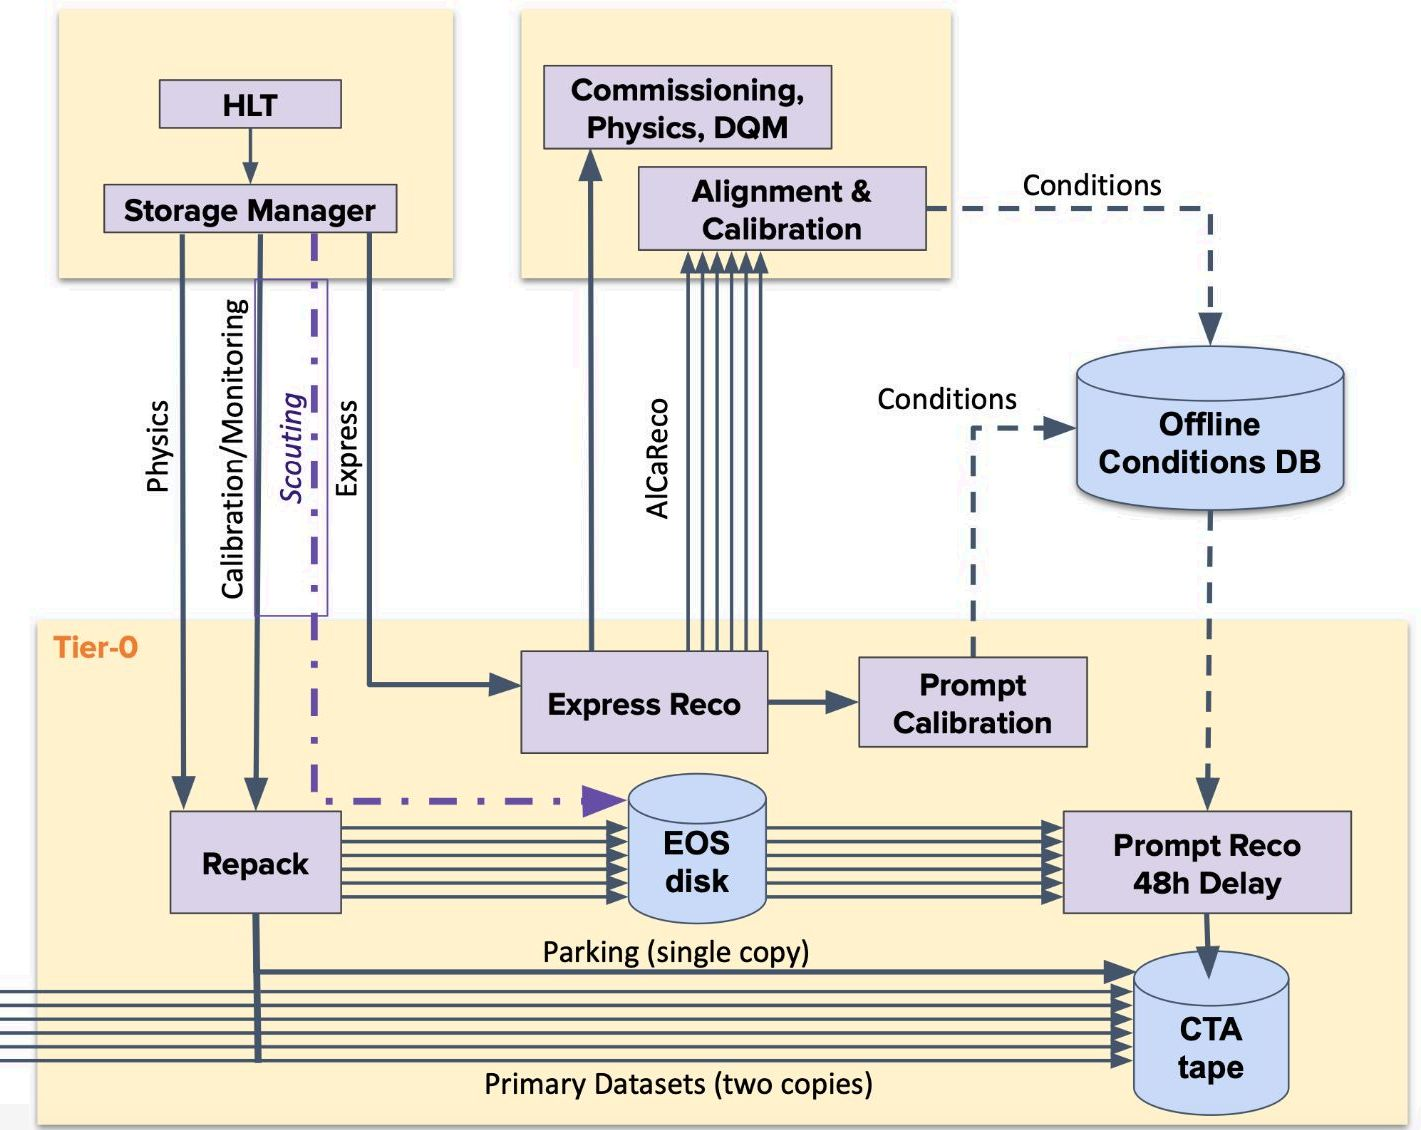
\includegraphics[width=\textwidth]{figures/PCL.jpg} %\hfill
\caption{Prompt Calibration Loop (PCL)}
\label{fig:PCL}
\end{figure}

\subsection{O2O}
\subsection{Other}

%%% Here we should add something about the automation framework






















































% The objective of \ngt{}'s \task{3.1.1} is to reconstruct all events received
% from the L1T at a rate of \SI{750}{\kilo\hertz} during Run-\num{5} data taking,
% eventually with an \emph{Offline-like} quality reconstruction. The
% reconstruction should enable some ``quick and dirty'' analyses using the
% reconstructed objects, without requiring additional steps. In order to
% understand where we are in terms of computing and physics performance, we
% decided to conduct a series of measurements using different scenarios, as
% explined in \ref{sec:measurements}. Considering a
% fixed budget for the farm in Run-\num{4} and Run-\num{5}, we need to determine
% the speed-up factor needed to be able to process the whole L1TA input rate with
% the required quality.
% 
% \section{Measurements}
% \label{sec:measurements}
% 
% As part of the first-year milestones, \task{3.1.1} is responsible for
% delivering a report on the performance of online reconstruction. This report
% will address identified bottlenecks, propose targeted improvements, and outline
% the necessary features for the generic CMS Structure of Arrays (\soa{}). To
% achieve this, we have begun conducting measurements using recent \CMSSW*{}
% releases. Our focus is on three specific performance metrics:
% 
% \begin{itemize}
% \item
%   \textbf{Measure the current performance of the \emph{simplified HLT Phase2
%     menu} for HL-LHC}: This will evaluate the present performance in terms of
%     computing speed and memory usage, with an aim to extrapolate these metrics
%     to 2030, the expected start of HL-LHC operations, and further down to 2032,
%     the beginning of Run-\num{5} operations. This will be done using both a
%     sample of \emph{TTbar} simulated events from the \textbf{Spring24} ongoing
%     campaign under 200PU conditions (and 140PU, if available), and a
%     specifically created \textit{skim} of L1 accepted events over an input
%     sample of \textit{MinimumBias} events, at 200PU.
% \item
%   \textbf{Assess the current performance of the \emph{offline Phase2
%     reconstruction}}: This will be done using both a sample of \emph{TTbar}
%     simulated events from the \textbf{Spring24} ongoing campaign under 200PU
%     conditions (and 140PU, if available), and a specifically created
%     \textit{skim} of L1 accepted events over an input sample of
%     \textit{MinimumBias} events, at 200PU. We will then project this
%     performance to 203{0,2}, considering anticipated improvements in CHF/HS06
%     and the likely shift of some algorithms and reconstruction processes to
%     accelerators. This analysis will help identify the necessary speedup factor
%     required to handle the full L1A rate directly during HLT processing using
%     an \textbf{offline-like reconstruction}, which is the final goal of this
%     task.
% \item
%   \textbf{Account for ongoing development in the \emph{offline Phase2
%   reconstruction}}: Since it is still evolving and lacks some
%   improvements present in the \emph{Run-3 reconstruction}, we also plan
%   to measure the performance of the \emph{Run-3 reconstruction} on a
%     simulated \textit{TTbar} sample with roughly 60PU. We will then identify which
%   modules from the \emph{Run-3 scenario} are missing in the
%   \emph{offline Phase2} sequence, estimate their
%   significance---particularly regarding CPU usage---extrapolate this
%   data to 200PU conditions, and incorporate it into our previous
%   performance measurements.
% \end{itemize}
% 
% All measurements have been done using \CMSSW[14][2][0][1]{}. A few additional patches have been necessary in order to correctly re-process the events. The patches fixed genuine bugs in the Phase\num{2} HLT Menu that were discovered while performing these measurements. Those patches have been submitted upstream to the main \CMSSW*{} release as pull requests (\href{https://github.com/cms-sw/cmssw/pull/46019}{46019} and \href{https://github.com/cms-sw/cmssw/pull/46054}{46054}) and integrated.
% 
% All samples used have been specifically produced to optimize the performance of the Phase\num{2} HLT reconstruction and of the offline reconstruction. Detailed instructions on how to create the samples and about their specificities are avaialble at \href{https://cms-ngt-hlt.docs.cern.ch/Task311/2024/Recipes/}{this link}\cite{ngt-recipes}.
% 
% Once all measurements are completed and the data is available, we will
% be in a better position to propose the next steps for development.
% Specifically, we will understand the extent of \textit{disruption} required to
% meet the highly ambitious goals outlined in this task.
% 
% \subsection{Pie resources}
% \label{subsec:pie-resources}
% 
% All pie-chart resources are usually available at
% \href{https://rovere.web.cern.ch/rovere/Phase2_HLT/circles/web/piechart.php}{this
% link}\cite{ngt-pies}. The measurements that are related to the \ngt{} project are
% usually collected under the \texttt{NGT\_\-Mea\-sure\-ments} folder.
% 
% \begin{nbbox}
% Some of the measurements collected at the link above are the results of several
% trials and errors. The measurements that are meant to be representative of each
% specific condition will be linked in the proper sections.
% \end{nbbox}

\chapter{Optimal Calibrations}
\section{General} % FIXME: the sections structure should be re-arranged/intergrated into the main general structure (the Introduction.tex part was untouched)

%% General
% From NGT Proposal: 
% This task will optimize the calibration process for the CMS detectors, from hours currently, to an online predictive model leveraging AI techniques. Such an improvement is essential to push real-time analysis based on R3 software (task 3.1) to the same accuracy that we typically achieve offline. One could then store high-quality high-level information, which implies a big save in terms of storage.

% Deliverable/milestone: Production of a report illustrating the current calibration workflows in CMS and evaluating the impact of non-optimal calibrations on the physics performance of the online reconstruction.

\begin{figure}[h!]	
\centering
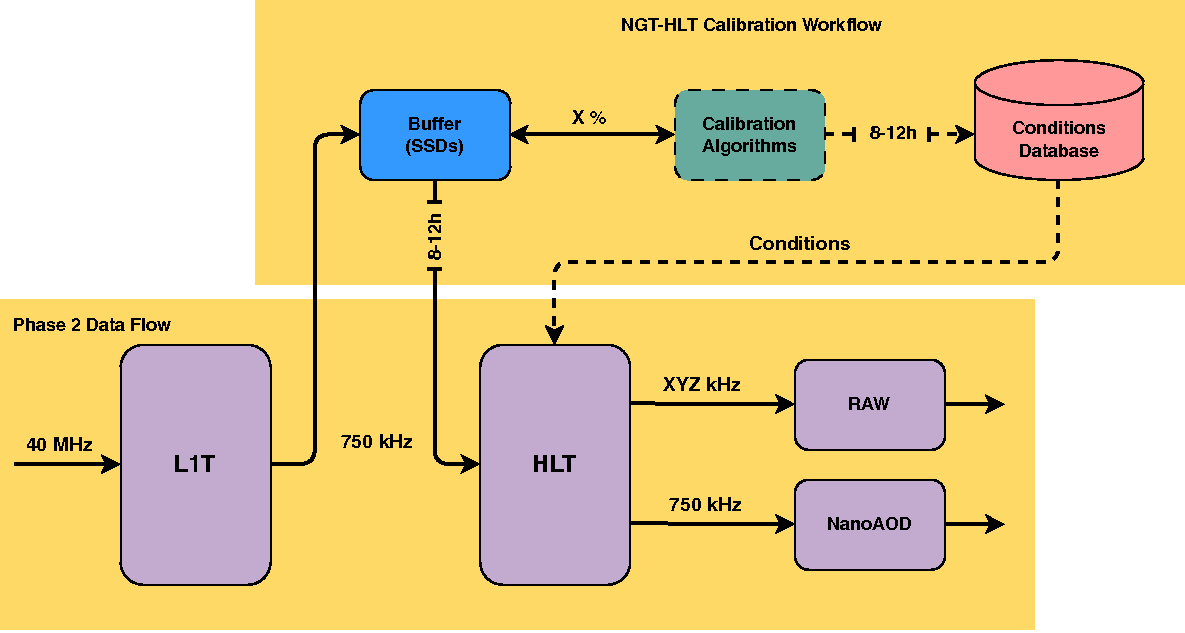
\includegraphics[width=\textwidth]{figures/NGT-HLT_Calibration_Workflow.drawio.pdf} %\hfill
\caption{Conceptual Design of $\mathrm{R}^{3}$ Optimal Calibrations (NGT-HLT Calibration Workflow)}
\label{fig:NGT-HLT_CalibrationWorkflow}
\end{figure}

\section{Calibration Workflows Analysis}
% Conduct a comprehensive analysis of the current calibration workflows and procedures within CMS currently in place, understanding the intricacies of the process, and identify areas for improvement (bottlenecks) in the calibration process. 

% NOTE: The current preliminary survey focused on finding viable candidates for the prototype. A continued and more detailed follow-up survey is being planned, especially in the context of Phase 2 calibrations, including new detectors (MTD, HGCAL, new tracker, etc.)

%\subsection{CMS Calibration Workflows}
% TODO: General introduction

% TODO: explain general AlCa: calibration vs condition, records, tags, etc.

% Latest GTs:
326 conditions (records/tags) in the latest HLT Global Tag (\texttt{140X\_dataRun3\_HLT\_v3}) used during LHC Run 3 p-p data taking in 2024.

% NOTE: Introduce prompt/offline in a similar manner?

\subsubsection{PCL}
\subsubsection{O2O}

⁄⁄‹\subsubsection{Other}
\subsection{Pixel Tracker Calibrations}

The CMS SiPixel detector is integral to the High-Level Trigger (HLT) decision-making process. This part of the report delves into the calibration prospects of the SiPixel detector, emphasizing unused records, FED cabling, gain and quality calibrations, CPE conditions, and alignment practices. Future prospects and recommendations for improving calibration workflows under the NGT framework are also discussed.
Out of the 326 conditions in the HLT GT, 13 are related to the Silicon Pixel Tracker, of which 12 are relevant to Run 3 data-taking. From these, the following 8 are considered core and critical for data-taking:

\begin{table}[h!]
    \centering
    \begin{adjustbox}{max width=\textwidth}
    \begin{tabular}{p{3.5cm}|p{4cm}|p{2.5cm}|p{2cm}|p{4.5cm}}
        \textbf{Name} & \textbf{Record} & \textbf{Workflow} & \textbf{Frequency of Updates} & \textbf{Description} \\ \hline
    \end{tabular}
    \end{adjustbox}
    \caption{Fundamental Silicon Strip Tracker Calibrations, ordered in terms of frequency of updates.}
    \label{tab:PixelCalibrations_critical}
\end{table}

\subsubsection{Unused Records in SiPixel Calibration}
Several records remain unused at HLT but hold relevance for other operational aspects:
\begin{itemize}
    \item \texttt{SiPixelDetVOffRcd}: Lists detector IDs with HV or LV off. Payload is ideal or empty.
    \item \texttt{SiPixelGainCalibrationOfflineRcd}: Stores gain and pedestal values for offline analysis.
    \item \texttt{SiPixelLorentzAngleRcd ("from alignment")}: Contains Lorentz Angle offsets, outdated since 2017.
    \item \texttt{SiPixelTemplateDBObjectRcd ("0T")}: Used during 0T templated tracking for PixelRecHits.
\end{itemize}

\subsubsection{FED Cabling and Calibration Maps}
The \texttt{SiPixelFedCablingMapRcd} records cabling maps connecting FEDs to readout channels. While not a direct calibration, this record plays a vital role in detector topology and reconstruction. This was last updated in 2017 with the transition to the Pixel Phase-1 detector.

\subsubsection{Bad components}
Description: This payload contains the DetIDs and ROCs associated with those DetIDs that are considered "dead." Used by tracking.\\
Record Name: \texttt{SiPixelQualityRcd} 

\subsubsection{Pixel Lorentz Angle}
Description: The 'no label' payload contains the value of LorentzAngle / Tesla for the Barrel Pixel and Forward Pixel separately (due to different HV constants, geometry, etc.).\\
Record Name: \texttt{SiPixelLorentzAngleRcd} 
Labels = none, \texttt{fromAlignment} or \texttt{forWidth} - given when included in a global tag.
\begin{itemize}
\item \texttt{fromAlignment} : the LA offset generated by alignment (alternative to LA correction from templates).
\item \texttt{forWidth}: the LA for charge width estimate in the generic CPE (alternative to the same LA as for offset). 
\end{itemize}

\subsubsection{Pixel Templates}
Description: used in the templated tracking algorithm for Pixel RecHits.
Record Name:  \texttt{SiPixelTemplateDBObjectRcd} 

\subsubsection{Generic Errors}

Description: used in the generic CPE (cluster position estimation) algorithm as errors. Improves irradiation bias corrections (IBC) for data.
Record Name:  \texttt{SiPixelGenErrorDBObjectRcd}

\subsubsection{Pixel Alignment}
Records used: 
\begin{itemize}
\item \texttt{TrackerAlignmentErrorRcd} (for alignment), 
\item \texttt{TrackerSurfaceDeformationRcd} (for surface deformation)  \item \texttt{GlobalPositonRcd} (defining the relative position of the subdetectors) 
\end{itemize}

Tracker alignment is tightly coupled with CPE conditions to mitigate Lorentz Angle miscalibrations. High-granularity offline PCL helps optimize biases but is prone to weak modes.
HLT reconstruction uses the Pixel CPE Fast algorithm (a variant of the generic algorithm), while offline operations rely on Pixel Template reconstruction. Discrepancies between these algorithms necessitate customized alignment procedures.

\begin{figure}[htbp]
   \centering
	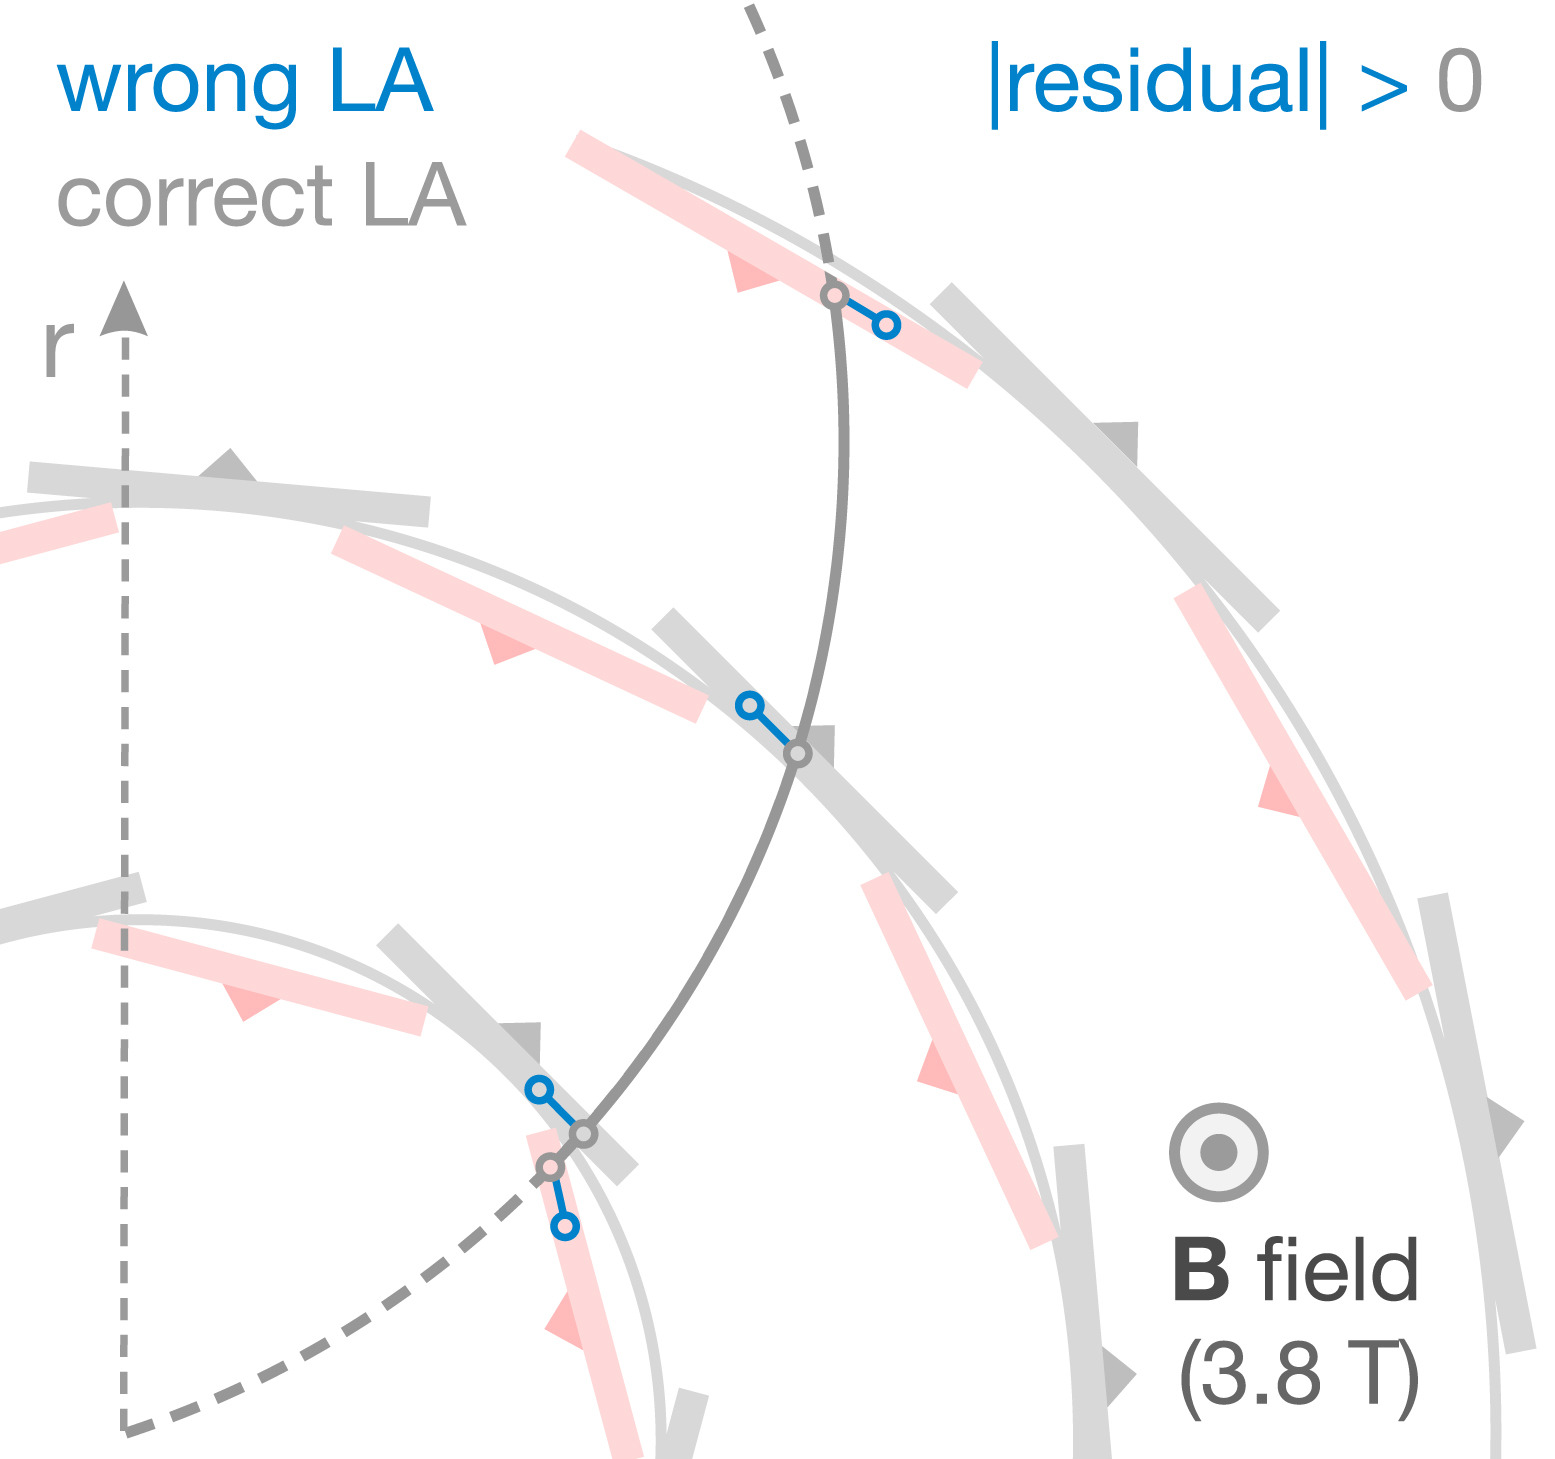
\includegraphics[width=0.5\textwidth]{figures/pixel_alignment_sketch.png}
   \caption{Sketch showing the transverse view of the Phase-0 barrel pixel subdetector, made of successive layers of silicon modules. The alternating orientation of the modules within each layer is indicated by the triangles. The blue (grey) circles represent the reconstructed hit positions using incorrect (correct) Lorentz angles in the presence of a magnetic field . The grey curve corresponds to a track built from the hits that were reconstructed with the correct Lorentz angles. Hits reconstructed with incorrect Lorentz angles are displaced in a direction defined by the orientation of the module, increasing the residual distance between the hits and the track. \cite{CMS:2022ali}}
   \label{fig:pixelAlignment}
\end{figure}

\subsubsection*{Future Prospects and Integration in NGT Demonstrator Workflow}
\begin{itemize}
    \item \textbf{Bad Components Masking}:
    \begin{itemize}
        \item Already implemented in PCL workflows and requires minimal statistics for updates.
        \item Demonstrated to improve track building in inside-out muon reconstruction.
    \end{itemize}
    \item \textbf{Pixel Alignment}:
    \begin{itemize}
        \item Enhancing alignment directly impacts B-tagging and physics trigger performance.
        \item Requires tailored workflows to address weak modes effectively.
    \end{itemize}
\end{itemize}

\subsubsection*{Recommendations}
\begin{itemize}
    \item Prioritize the inclusion of bad components masking in the NGT demonstrator workflow due to its operational simplicity and demonstrated impact.
    \item Develop alignment calibration workflows that directly integrate HLT tracks to ensure compatibility.
    \item Evaluate the feasibility of frequent updates for gains and CPE conditions to maintain precision.
\end{itemize} % Marco
\subsection{Strip Tracker Calibrations}

Out of the 326 conditions in the HLT GT, 24 are related to the Silicon Strip Tracker, of which 21 are relevant to Run 3 data-taking. From these, the following 4 are considered core and critical for data-taking:

\begin{table}[h!]
    \centering
    \begin{adjustbox}{max width=\textwidth}
    \begin{tabular}{p{3.5cm}|p{4cm}|p{2.5cm}|p{2cm}|p{4.5cm}}
        \textbf{Name} & \textbf{Record} & \textbf{Workflow} & \textbf{Frequency of Updates} & \textbf{Description} \\ \hline
    \end{tabular}
    \end{adjustbox}
    \caption{Fundamental SiStrip Calibrations, ordered in terms of frequency of updates.}
    \label{tab:StripCalibrations_critical}
\end{table}

\subsubsection{DAQ O2O conditions}

\subsubsection{DCS O2O conditions}

\subsubsection{Bad Components}

\subsubsection{APV gains}

\subsubsection{CPE conditions}

\subsection{Others} % Marco
%!TEX root = ../main.tex
\subsection{ECAL Calibrations}

%%% I don't know how much I believe these numbers here.
Out of the 326 conditions in the HLT GT,
67 are related to ECAL, %59 
of which 52 are relevant to \Runthree data-taking. %36
From these, the following are considered core and critical for data-taking:
\begin{table}[h!]
    \centering
    \begin{adjustbox}{max width=\textwidth}
    \begin{tabular}{p{3.5cm}|p{4.5cm}|p{2.5cm}|p{2cm}|p{4cm}}
        \textbf{Name} & \textbf{Record} & \textbf{Workflow} & \textbf{Frequency of Updates} & \textbf{Description} \\ \hline
    Laser corrections & \texttt{EcalLaserAPDPNRatios} & ECAL automation and manual & Every 40 min or per fill & Crystal transparency and photodetector response. \\
    Pedestals & \texttt{EcalPedestals} & PCL and ECAL automation & Per run or weekly & Pedestals for noise measurements. \\
    Pulse shapes & \texttt{EcalLaserAPDPNRatios} & ECAL automation and manual & 3 days & Pulse shapes. \\
    Timing & \texttt{EcalTimeCalibConstants} & ECAL automation and manual & Weekly & Time of the pulse maximum.\\
    Intercalibrations & \texttt{EcalIntercalibConstants} & ECAL automation and manual & Weekly or more & Equalise crystal response vs. $\eta$ and $\phi$.
    \end{tabular}
    \end{adjustbox}
    \caption{Fundamental ECAL Calibrations, ordered in terms of frequency of updates.}
    \label{tab:ECALCalibrations_critical}
\end{table}

\subsubsection{Pedestals}

%EcalPedestalsRcd

The ECAL pedestals represent the baseline from which the electronics pulses are measured.
Pedestals are measured for the three possible configurations (gains) of the multi-gain preamplifier integrated in the ECAL readout chip: $\times 1$, $\times 6$ and $\times 12$.
In the offline tag, 
the PCL updates the G12 pedestals automatically, while
the G1 and G6 pedestals are updated manually every week.
In the online tag, all three pedestals are updated manually weekly.

\subsubsection{Laser Corrections}

%EcalLaserAPDPNRatiosRcd

The transparency of the ECAL crystals and the photodetector's response to light are degraded as an effect of the irradiation from the LHC collisions.
The degradation as a function of time is monitored crystal by crystal by measuring the response to the light of a laser system.
The light is injected in the system during the LHC abort gap, and a complete scan of the calorimeter takes 40 minutes.
The measurement of the response degradation is then used as a correction factor in the energy reconstruction.
In the offline tag, this correction is available with that same 40-minutes granularity,
while in the online tag it is available only once per LHC fill.

\subsubsection{Pulse Shapes}

%EcalPulseShapesRcd

The ECAL pulse shapes also change because of the irradiation affects,
and those changes also directly change the reconstruction of the signal amplitude.
These updated are more critical after a technical stop of the LHC.
The same payloads are used in the offline and online tags.

\subsubsection{Timing Corrections}

%EcalTimeCalibConstantsRcd

The ECAL timing drifts 
towards negative times during collisions 
and
towards positive times during recovery.
For the current standard used for the calibration (ratio timing), 
the same payloads are used in the offline and online tags.

\subsubsection{Intercalibrations}

%EcalIntercalibConstantsRcd

The intercalibrations are derived for each crystal and employ a series of methods:
the azimuthal symmetry of the energy deposits in ECAL,
the known mass of particles that decay to electrons and photons
($\text{Z}\to\text{ee}$, $\pi^0\to\gamma\gamma$),
and
the energy--momentum ratio ($E/p$) of electrons from electroweak boson decays.
In general these calibrations require multiple inverse femtobarns of integrated luminosity to derive;
the same payloads are used in the offline and online tags.

\subsubsection{Alignment}

Alignment of the ECAL with respect to the Tracker system is done infrequently, 
mainly when there is a cycle of the CMS magnet.

In view of the above discussion, we consider the \emph{laser corrections} a possible candidate for the implementation in NGT.
The gap between online and offline update frequencies (40 minutes vs. per fill) is large enough that, in principle, expressive improvements can be realised by improving the online calibration. % Thiago
\subsection{HCAL Calibrations}

The calibration of the hadron calorimeter\footnote{Details of the detector are presented in \ref{CMS}} (HCAL) is vital in the determination of the energy scale and resolution of hadrons, and consequently jets and missing transverse momentum.

There are no HCAL calibrations included in the PCL, however, there exist HCAL automation workflows that update HCAL conditions on a weekly basis (e.g. gains, pedestals). Most conditions are explicitly baked into the Look-Up Tables (LUTs) that are loaded on-detector and append the GT via the O2O procedure semi-automatically. The remaining conditions are uploaded manually to the conditions database. Many HCAL conditions are also relevant for L1T and the corresponding trigger primitives. Out of the 326 conditions in the HLT GT, 37 are related to HCAL, of which 24 are relevant to Run 3 data-taking. From these, the following 9 are considered core and critical for data-taking:

\begin{table}[h!]
    \centering
    \begin{adjustbox}{max width=\textwidth}
    \begin{tabular}{p{3.5cm}|p{4cm}|p{2.5cm}|p{2cm}|p{4.5cm}}
        \textbf{Name} & \textbf{Record} & \textbf{Workflow} & \textbf{Frequency of Updates} & \textbf{Description} \\ \hline
        Gains (RadDam) & \texttt{HcalGains} & O2O & Weekly & Response corrections for radiation damage (RadDam). \\
         Pedestals & \texttt{HcalPedestals} & HCAL automation (O2O) & Weekly & Pedestals for noise measurements.
measurements.\\
        Pedestal Widths & \texttt{HcalPedestalWidths} & HCAL automation (O2O) & Weekly & Pedestals for noise measurements.
measurements. \\
        L1T Trigger Objects & \texttt{HcalL1TriggerObjects} & HCAL automation (O2O) & Weekly & L1T trigger objects, including relevant conditions: pedestals, gains and response corrections, channel quality. \\
        Response Corrections & \texttt{HcalRespCorrs} & O2O & per Era ($\approx 20~\fbinv$) & Corrections to detector energy response. \\
        Channel Quality & \texttt{HcalChannelQuality} & O2O & Few times per year & Tracking dead or non-functional HCAL cells. \\
        Geometry Parameters & \texttt{HcalParameters} & Manual & Yearly & Parameters related to the HCAL geometry. \\
        Look-Up Tables (LUTs) & \texttt{HcalLUTCorrs} & O2O & Rarely & Corrections related to Look-Up Tables (LUTs). \\
    \end{tabular}
    \end{adjustbox}
    \caption{Fundamental HCAL Calibrations, ordered in terms of frequency of updates.}
    \label{tab:HCALCalibrations_critical}
\end{table}

In the context of an optimal calibrations workflow, the first 6 from Table \ref{tab:HCALCalibrations_critical} are considered fundamental\footnote{There exist fundamental HCAL conditions or calibrations which can have a significant effect on HLT reconstruction that are implemented in the hardware directly (e.g. timing alignment, zero-suppression thresholds, \texttt{HcalZSThresholds}) while their conditions database records may not be considered critical per se (but rather used for bookkeeping purposes).} and generally require more frequent updates. These have been analysed in more detail in the following sections. % NOTE: footnote could be moved to Others section.

\subsubsection{Response Corrections}
Response corrections are calibrations that aim to equalise the signal coming from the detector to provide a uniform energy measurement. They have a very significant effect on HLT reconstruction and rates, and thus are considered critical. Generally, they are updated roughly every era ($\approx 20 \fbinv$), however, the exact frequency depends on the HCAL subsystem and type of correction. Generally, the required statistics determines the frequency, as the analyses are often statistically limited. Technically-speaking, if the calibrations are determined accurately, they would require less-frequent updates (modulo hardware changes). The updates are explicitly baked into the LUTs that are loaded on-detector and the corresponding conditions appended to HLT GT via the O2O procedure semi-automatically.

% HB and HE
The main calibrations for the HB and HE come in in two forms: azimuthal ($\phi$\texttt{-symmetry}) and isolated track (\texttt{IsoTrack}) corrections, which are multiplicative factors. 

% Azimuthal (Phi-)Symmetry
Asymmetries in the response over $\phi$ arise due to structure, materials, inhomogeneous magnetic field, beam-spot shifts, and miscalibrations. The $\phi$\texttt{-symmetry} intercalibrations equalize the detector response in $\phi$ for each $i\eta$ ring and depth section of the HCAL. They take advantage of the uniformity of particle energies across the azimuthal angle $\phi$. An intercalibration is performed between calorimeter channels by comparing it to the average collected energy in the entire $i\eta$ ring. Two methods are used to determine them, depending on the hadron energies:
\begin{itemize}
    \item For high energies ($> 4 \GeV$) an iterative method is used, where scale factors for uncalibrated energies are determined iteratively by equalizing the mean of the energies in an energy interval. An unbiased dataset is used with events triggered by detectors other than HCAL, such as electron, photon and muon triggers. The reconstructed energies are obtained from zero-suppressed events after noise (pedestal) subtraction.
    \item For low energies ($< 4 \GeV$; down to a fraction of a GeV), a method of moments is used, where the first (mean) and second (variance) moments of the energy distribution are compared to that of the entire $i\eta$ ring. This method uses minimum-bias events taken without zero-suppression (NZS). The noise (pedestal) is subtracted from the energy distribution.
\end{itemize}

The uncertainty-weighted average of the scale factors from both methods is used as the final scale factor for the $\phi$-intercalibration.

% Isolated Track (IsoTrack)
An absolute calibration of charged hadrons is performed by comparing the energy measurement with that of the tracker system, taking advantage of the precise calibration of the tracker system. Unlike the tracker momentum measurement, the HCAL energy response is non-linear, especially at lower energies. Therefore, the goal of the calibration is to equalize the relative energy scale for higher momentum charged hadrons that do not interact hadronically with the ECAL. Isolated tracks of hadrons with momenta between $40-60 \GeV$ are used. Data samples are collected using dedicated \texttt{IsoTrack} triggers with special isolation and maximum requirements on the energy deposited in the ECAL, as well as a more standard set of physics triggers with similar selections applied offline. Assuming there are no statistical limitations, preferably they are determined in a depth-dependent way, which is more optimal.

% HF
The forward calorimeter (HF) is also calibrated using the $\phi$-symmetry, while the energy scale is extrapolated using $Z \rightarrow ee$ events. The dataset consists of events with one electron candidate in the HF and the other in the ECAL, which has been precisely calibrated. The scale is adjusted so that the dielectron invariant mass corresponding to the Z-peak is consistent between data and simulation.

% HO, ZDC
For HO, the intercalibration makes use of muons from collision data, as well as cosmic ray muons, while the determination of the absolute energy scale makes use of di-jet events. These calibrations are mostly unchanged with respect to initial calibrations.

The Zero-Degree Calorimeter (ZDC) calibrations are also mostly unchanged and are not discussed here further. 

% NGT candidate assessment
In the context of a potential candidate for the optimal NGT calibrations, it is clear that the response corrections involve a number of dedicated separate offline analyses for different HCAL subsystems, using various input datasets (incl. \texttt{AlCaRecos}) and specific selections. Thus, their determination is rather convoluted and they are tricky to do without proper offline analysis and corresponding validation. Even though some of the sub-calibrations might be reasonably possible to automate (e.g. $Z \rightarrow ee$ for HF), it would still require significant work to automate. Furthermore, since they are baked into the LUTs, they are entangled together with L1T condition updates. Therefore, one can conclude that the response corrections are not a viable candidate for the NGT workflow in their current form, especially for the Run 3 prototype.

\subsubsection{Gains (RadDam)}\label{sec:HCAL_gains}
The  \textit{gains} (or \texttt{RadDam}) calibrations are responsible for correcting for radiation damage in the HCAL. Generally this leads to a decreased signal due to the darkening of active scintillator material and fibres (similar to the ECAL laser corrections covered in Section \ref{sec:ECALlaser}). Conversely, the recovery process of thermal annealing also effects the signal and needs to be corrected for. Due to the increased radiation in the forward region, primarily HE and HF are corrected. These corrections are especially important in the high $|i\eta|$ regions where there is no tracker coverage and the \texttt{IsoTrack} response corrections are less accurate and cannot cover for these differences. Therefore, they can be considered critical especially for those regions. HB and HO have not been corrected for a long time due to lower radiation damage. The corrections are determined $|i\eta|$- and depth-dependent and $|i\phi|$-independent) yielding a multiplicative factor together with the response corrections for final calibrated response in GeV. Generally, they are updated via the O2O procedure semi-automatically (as with the response corrections) roughly every era ($\approx 20 \fbinv$).

Typically, the measurements of the radiation damage is based on laser data in the orbit/abort gap, when there is no beam in the LHC. The laser system sends light to the photodetectors (SiPMs, PMTs) or directly to the scintillators. The ratio of the amplitudes gives a measure of the signal attenuation. The laser data is then compared to that taken at the start of the yearly data-taking in order to measure the net effects of radiation damage. A new dedicated radiation damage monitoring system was recently developed for the HF quartz fibres. 

The effects of radiation damage are dependent on the delivered luminosity. The dependence is modelled and parametrised to exponential decay \cite{CMS-PRF-18-003}. An example of the relative laser signal in a single $i\eta$ region and layer is shown in Figure \ref{fig:ECAL-Laser_data}. 

\begin{figure}[h!]	
\centering
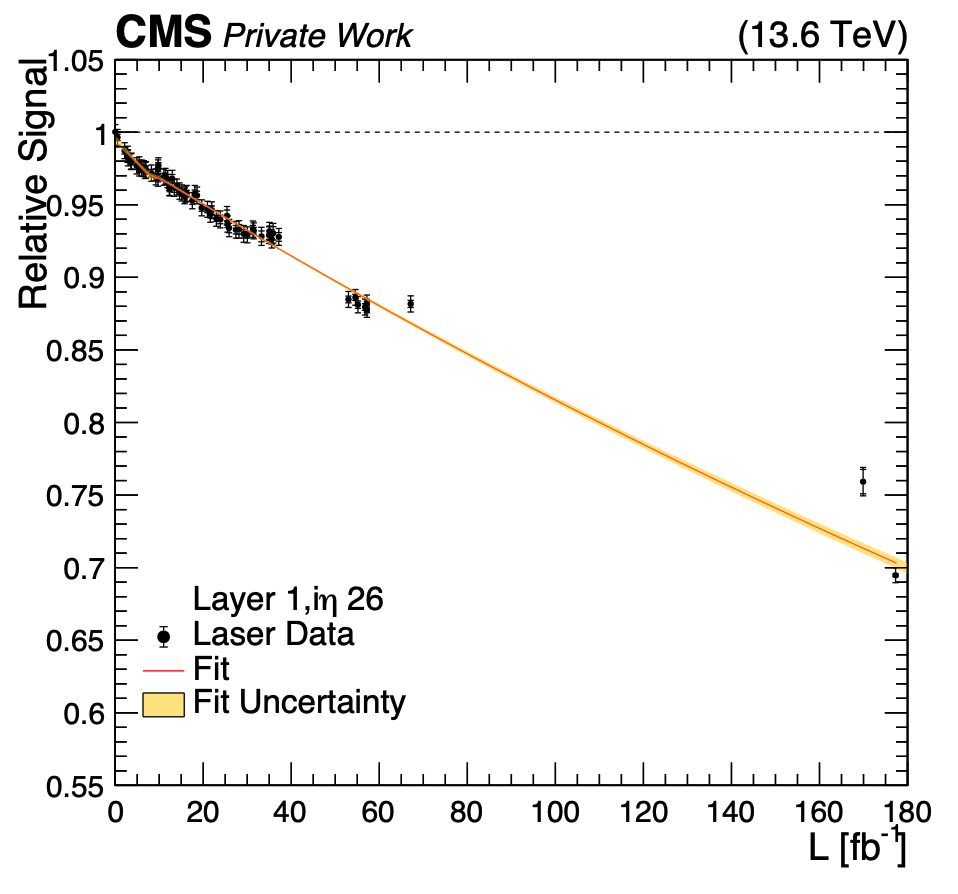
\includegraphics[width=0.7\textwidth]{figures/HCAL-Laser_data2024.png} %\hfill
\caption{Laser system data in layer 1, $i\eta = 27$ of the HCAL, indicating the relative signal as a function of the total integrated luminosity L in $\fbinv$, parametrised as exponential decay. The missing data points indicate the extended downtime of the laser system in 2024.}
\label{fig:HCAL-Laser_data}
\end{figure}

In the case of downtime of the laser system (also seen in Figure \ref{fig:ECAL-Laser_data} for 2024), the backup approach are dedicated energy flow extrapolations, which are non-trivial. Therefore, the preference is to use laser data.

% NGT candidate assessment
In the context of a potential candidate for the optimal NGT calibrations, the gains or \texttt{RadDam} corrections are important for HLT reconstruction and require frequent updates. There are plans to include them in the HCAL automation system (covered in more details the next Section \ref{sec:HCAL_pedestals}) within weekly updates. Therefore, they are a good candidate for the NGT workflow. One caveat is that they are dependent on laser data, which requires different data stream than the standard bulk collisions data. Furthermore, a vital requirement is a well-functioning laser system.

\subsubsection{Pedestals}\label{sec:HCAL_pedestals}
The HCAL pedestals and their corresponding widths are essentially measurements of the noise "floor" that are offset to avoid any energy measurement bias. Generally-speaking, noise increases with radiation damage. Regular pedestal updates are important to avoid any drifting of HCAL-driven trigger rates and contributions to the fraction of the energy deposited in the HCAL and ECAL, $\frac{H}{E}$, which is an observable used in the identification of electrons and photons, including shower shapes and isolation. The pedestals are also important inputs into other calibrations, such as the response corrections.

Generally, they are updated roughly every week ($\approx 2 \fbinv$), as part of the HCAL automation workflow. The workflow is used to calculate effective pedestals from collision runs, where good input data from candidate runs is identified and processed within 1 hour after a given LHC fill. The input data is based on measurements in orbit/abort gap when there is no beam in the LHC (similarly to the laser data for the HCAL gains discussed in the previous Section \ref{sec:HCAL_gains}). The conditions are automatically uploaded to the conditions database via the O2O procedure. Validation in the context of changes to L1T and HLT trigger rates are produced within 2 hours, with an ultimate validation and green-light from AlCa typically after 1-2 days. Given a successful validation, this is followed by deployment at the subsequent LHC interfill period.

% NGT candidate assessment
In the context of a potential candidate for the optimal NGT calibrations, the pedestals are critical inputs. The are included in the HCAL automation system within weekly updates, which automatically make them a good candidate for the NGT workflow. One caveat is that they are dependent on orbit/abort gap data, which requires different data stream than the standard bulk collisions data.

% \subsubsection{Others}

% NOTE: more complete list in annex? e.g. non-critical calibrations % Mateusz
%!TEX root = ../main.tex
\subsection{Muons System Calibrations}

Out of the 326 conditions in the HLT GT,
41 are related to the muon systems:
14 to the Drift Tubes (DTs),
20 to the Cathode Strip Chambers (CSCs),
and
7 to the Resistive Plate Chambers (RPCs).
No conditions are related to the Gas Electron Multipliers (GEMs) as of 2024,
and
the RPCs don't have calibrations that can affect the data quality.
The only conditions that are considered core for data-taking are:
\begin{table}[h!]
    \centering
    \begin{adjustbox}{max width=\textwidth}
    \begin{tabular}{p{3.5cm}|p{4.5cm}|p{2.5cm}|p{2cm}|p{4cm}}
        \textbf{Name} & \textbf{Record} & \textbf{Workflow} & \textbf{Frequency of Updates} & \textbf{Description} \\ \hline
    DT drift velocity & \texttt{DTMtime} & Manual & Rarely & Drift velocity of the ionisation electrons. \\ 
    DT timing offset & \texttt{DTTtrig} & Manual & Yearly & Timing offset of the ionisation electrons. \\ 
    CSC time corrections 	& \texttt{CSCChamberTimeCorrections} & Manual & Yearly & Adjustments to center reco. hit times at $t=0$. \\
    						& \texttt{CSCDBChipSpeed} & Manual & Rarely & \\ 
	CSC electronics & \texttt{CSCDBGains} & Manual & Yearly & Electronics parameters of strips channels. \\
                    & \texttt{CSCDBPedestals} & Manual & Yearly &  \\
					& \texttt{CSCDBCrosstalk} & Manual & Yearly &  \\ 
                    & \texttt{CSCDBNoiseMatrix} & Manual & Yearly &  \\
    \end{tabular}
    \end{adjustbox}
    \caption{Fundamental Muon System Calibrations, ordered in terms of frequency of updates.}
    \label{tab:MuonCalibrations_critical}
\end{table}

In all conditions related to the muon systems, all workflows are manual, the frequency of updates is small, and payloads are always kept the same between online and offline.
As such, we conclude that the muon system doesn't provide any candidate conditions for the NGT project.
 % Thiago

\section{Physics Performance}

%%% Here we discuss the 
%% Physics performance
% Assessment on the impact of non-optimal calibrations on the physics performance of the online reconstruction, by analysing data to quantify the effects of calibration inaccuracies.

%!TEX root = ../main.tex
\section{NGT--DAQ Integration} % Thiago

%%% We just write the discussion we had in the whole DAQ session

The Optimal Calibration system has to be embedded in the CMS trigger and data acquisition (DAQ) system,
both in the demonstrator system and in the Phase-2 implementation.
We briefly discuss the DAQ system architecture implemented for Run 3, 
and how the demonstrator can be inserted in that system.
We then review the conceptual DAQ design proposed for Phase-2, and 
go through a preliminary calculation of the NGT system feasibility.

\subsection{Demonstrator Integration in Run 3}

The CMS DAQ system for Run 3 (DAQ3) is an intricate system, dealing with all steps of the data flow from the sub-detector front-end drivers (FEDs) through the final delivery of data streams to Tier-0. For the purposes of our discussions, we can focus on the following elements of Figure~\ref{fig:DAQ3}: 
the \emph{Readout Units} (RUs) unpack and merge event fragments into super-fragments, which are then sent to the \emph{Builder Units} (BUs) to be further assembled into complete events. 
The complete events are sent to the \emph{Filter Units} (FUs), where the HLT application runs and selects a subset of the events to be saved for permanent storage. 
In the DAQ3 implementation, the RUs and the BUs are logically separate, but physically realised in the same computer node.
\begin{figure}[htbp]
   \centering
	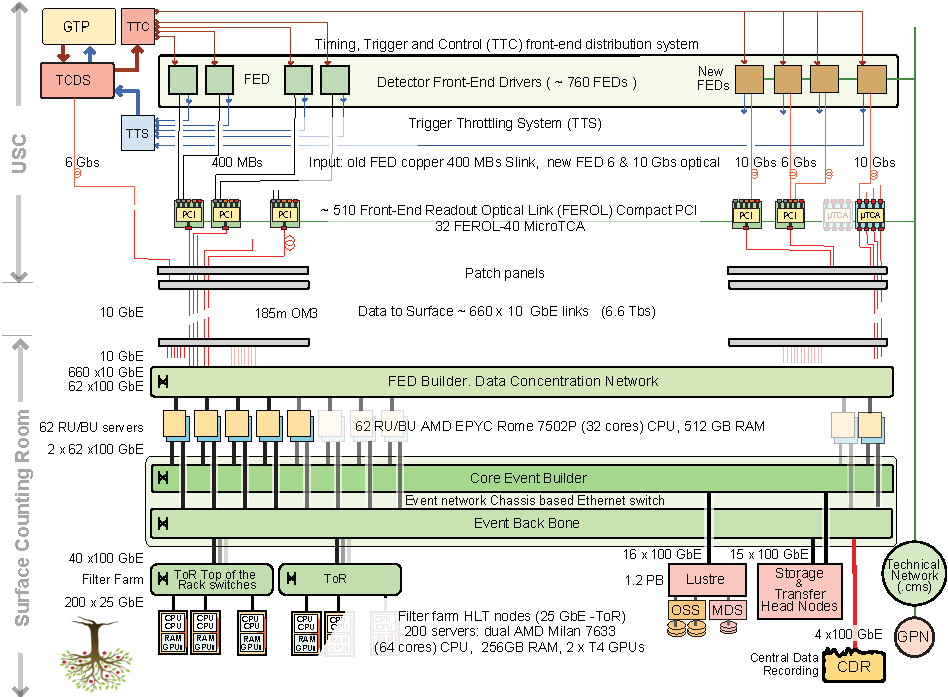
\includegraphics[width=0.7\textwidth]{figures/DAQRun3.pdf}
  \caption{Diagram of the Run 3 DAQ system.}
   \label{fig:DAQ3}
\end{figure}

The output data are then sent back to the BUs, where they are further merged and their management is handed over to the storage and transfer system (STS).
The STS  transfer the data to a (Lustre-based) cluster file system, whence they are finally sent to their final destination:
Tier-0,
DQM
or the calibration cluster.
The DAQ3 was also designed with two characteristics that the demonstrator should respect: 
i) it is \emph{pipelined}, so the data should follow an unidirectional flow;
ii) it is \emph{democratic}, in the sense that all elements (RUs, BUs, FUs) are treated equally.

%%% Thiago testing the GitHub integration
% I want to work at the LHC!
% I want to work at the FCC!

\subsection{Conceptual DAQ Design for Phase-2}

\subsection{System Feasibility: Preliminary Calculation}

As the overarching goal of the NGT project is to reconstruct and save all the L1-accepted data, 
our first assumption is that the system will have to buffer all the data of a run whilst 
running the optimal calibrations.
The size of the data buffer $B$ can be estimated by the following formula
\begin{equation}
B = A^{\text{L1}} \times \tau \times E \times s
\label{eq:buffersize}
\end{equation}
where $A^{\text{L1}}$ is the Level-1 trigger accept rate,
$\tau$ is the period during which we have to buffer the data,
$E$ is the event size and
$s$ is a safety factor.
For a first calculation, we take the Run 4 estimates from the DAQ-HLT TDR:
-- $L1A$ = 500\kHz, $E$ = 6.1\,MB --
and assume a flat 50\% safety factor ($s$ = 1.5).
The discussion on the magnitude of the buffer period $\tau$ is more subtle and will be done in the next section.

\subsubsection{Buffer Period}

The amount of time during which the data has to be buffered depends on many factors,
and we add a set of working hypotheses to be able to estimate its value.
\begin{itemize}
\item The buffer period has to be longer than the amount of time needed to derive the calibrations.
A relevant timescale is the PCL completion time, which we know from experience to take close to eight hours.
We know from experience that the PCL takes, in average, 8 hours to run for completion.
Some of the longest runs, however, may need additional time; a long run from LHC fill 10200 took data during more than 13 hours
(delivering close to $900\pbinv$), and
the PCL took more than 10 hours to finish,
as seen in Fig.~\ref{fig:fill10200PCL}.
Notice that, in offline reconstruction, Tier-0 starts the PCL only after the run end; 
therefore the 48 hours limit for the start of prompt reconstruction applies to 
the sum of run duration and the PCL duration.
After the calibration is done the data has to be buffered for some more time in order to allow the NGT reconstruction to run.
Therefore, we choose to use a representative value of \emph{12 hours}.
\begin{figure}[htbp]
   \centering
	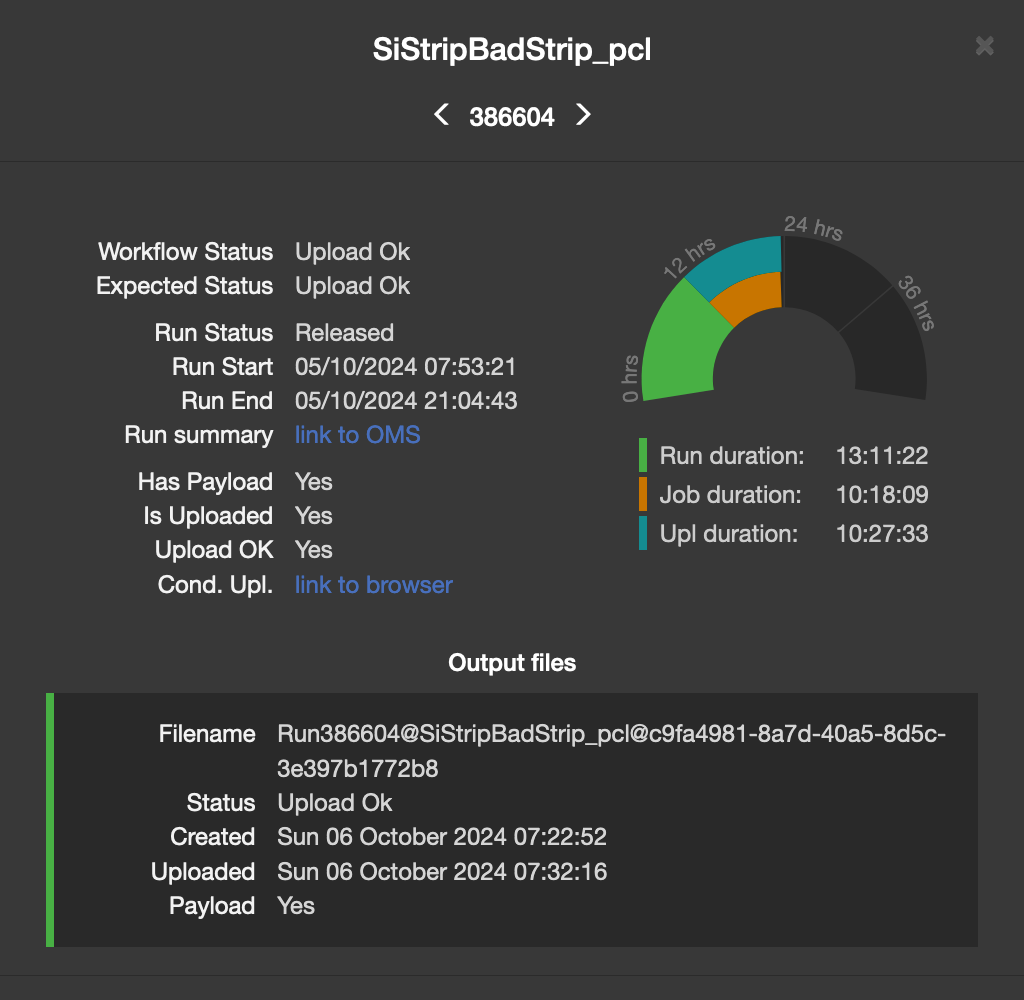
\includegraphics[width=0.7\textwidth]{figures/fill10200PCL.png}
   \caption{PCL monitoring of the silicon strip bad components calibration for a run of LHC fill 10200 (the number 386604 refers to internal CMS bookkeeping).
   The run took data over more than 13 hours, whilst the PCL ran for over 10 hours.}
   \label{fig:fill10200PCL}
\end{figure}
\item On the other hand, the buffer has to be large enough to store all the data from an LHC fill, as per our first assumption,
but that calculation has to take into account the LHC duty cycle, so we use the following working hypotheses:
\begin{itemize}
\item The High-Luminosity LHC will work in a $\sim70\%$ duty cycle, meaning that in a 24-hour period there will be 17 hours of stable beams and 7 hours of interfill (including injection and ramp).
\item Levelling will once again be used to keep the effective luminosity at a given level.
Following the Run 3 historic performance, we assume that the 17 hours of stable beams will be divided into 10 hours of levelling and 7 hours of lumi decay phase.
\item Again following the Run 3 performance, we assume that the luminosity (as well as the pileup) in the decay phase will average out to $\sim80\%$ of levelled luminosity.
\item We assume that the event size $E$ scales linearly with pileup.
\item We assume that the Level-1 accept rate $L1A$ will be kept constant even during the decay phase. 
\item The 7 hours of downtime are effectively free from the point of view of data buffering for NGT.
\end{itemize}
\end{itemize}

By simply substituting $\tau$ = 12 hours in Eq.~\ref{eq:buffersize}, we arrive at a buffer size $B$ = 200 PB.
The second calculation that accounts for the LHC duty cycle amounts to three applications of the same equation,
and is summarised in Table~\ref{tab:bufferWithDutyCycle}. In that case, we arrive at a buffer size of $B$ = 258 PB for a 24 hour period.
Noting that the two results agree within $\sim25\%$, and that many more assumptions go into the second calculation, for the purposes of this report we proceed with the \textbf{200\,PB} figure.
% Requires the booktabs if the memoir class is not being used
\begin{table}[htbp]
   \centering
   %\topcaption{Table captions are better up top} % requires the topcapt package
   \begin{tabular}{@{} lrrrrr @{}} % Column formatting, @{} suppresses leading/trailing space
      \toprule
		Phase & Duration (h) & $A^{\text{L1}}$ (kHz) & $E$ (MB) & Safety factor & Buffer (PB)\\
      	\midrule
		Levelling & 10 & 500 & 6.1 & 1.5 & 165 \\
		Decay     &  7 & 500 & 4.9 & 1.5 &  93 \\
		Interfill &  7 &  -- &  -- &  -- &   0 \\
		\midrule
\textbf{Total}    & \textbf{24} & N/A & N/A & N/A & \textbf{258}\\ 
      \bottomrule
   \end{tabular}
   \caption{Calculation for NGT buffer size accounting for LHC duty cycle. 
   This modelling concludes that a 258\,PB buffer is adequate for a 24-hour period.}
   \label{tab:bufferWithDutyCycle}
\end{table}

We can compare the proposed NGT buffer size to a number of similar systems.
The current storage capacity of the CMS Run 3 DAQ system is 1.2\,PB.
The LHCb experiment implemented a similar dataflow in their DAQ system, 
with events accepted by their HLT1 system held in a 30\,PB buffer,
used for real-time alignment and calibration,
and finally passed on to their HLT2 system.
\textcolor{red}{Lastly, the CMS Tier-0 holds a disk buffer of 11\,PB for incoming raw data from Point 5 to be held on for prompt reconstruction,
as well as a disk buffer of 25\,PB for reconstructed data before it is transferred to other sites in the WLCG.}
We also note that experience from the LHCb system shows that the reading/writing speed of the disks decreases when they fill up,
which justifies the consideration of a large safety factor ($s = 1.5$).

\subsubsection{Nodes for the Optimal Calibration}

The computer nodes for the optimal calibration have to be integrated in the DAQ system.
The alignment and calibration algorithms need built events to run over, so these nodes need to be downstream of the BUs.

\subsubsection{Additional Output from NGT Workflow}





\chapter{Conclusions and Outlook}
% TODO: add that a continued and more detailed follow-up survey is being planned, especially in the context of Phase 2 calibrations, including new detectors (MTD, HGCAL, new tracker, etc.)

\printbibliography % Print the bibliography

\end{document}
